\documentclass[12pt,a4paper,titlepage,final]{article}
\usepackage[czech]{babel}
\usepackage[utf8]{inputenc}
\usepackage[bookmarksopen,colorlinks,plainpages=false,urlcolor=blue,unicode]{hyperref}
\usepackage{url}
\usepackage{float}
\usepackage{ifthen}
\usepackage[dvipdf]{graphicx}
\usepackage[top=3.5cm, left=2.5cm, text={17cm, 24cm}, ignorefoot]{geometry}

\begin{document}
\newpage

%%%%%%%%%%%%%%%%%%%%%%%%%%%%%%%%%%%%%%%%%%%%%%%%%%%%%%%%%%%%%%%%%%%%%%%%%%%%%%
% titulní strana
\def\name{Lukáš Vokráčko}
\def\login{xvokra00}
\def\subject{Paralelní a distribuované algoritmy}
\def\project{Carry Look Ahead Parallel Binary Adder}

\newboolean{frontpage}
% \setboolean{frontpage}{true}
\setboolean{frontpage}{false}

\ifthenelse{\boolean{frontpage}}
{
	\pagestyle{empty}
	\input{title.tex}
	\tableofcontents
	\newpage
	\pagestyle{plain}
}
{
	\pagestyle{plain}
	% \vspace*{2px}
	\hfill \name, \login \\
	\vspace*{5px}
	{\LARGE \subject}  \\
	{\LARGE \project}  \\
}

\pagenumbering{arabic}
\setcounter{page}{1}
%%%%%%%%%%%%%%%%%%%%%%%%%%%%%%%%%%%%%%%%%%%%%%%%%%%%%%%%%%%%%%%%%%%%%%%%%%%%%%

\section{Analýza algoritmu}

\section{Implementace}
Program je implementován v jazyce C++ s využití knihovny \url{https://www.open-mpi.org/}.

\section{Experimenty}
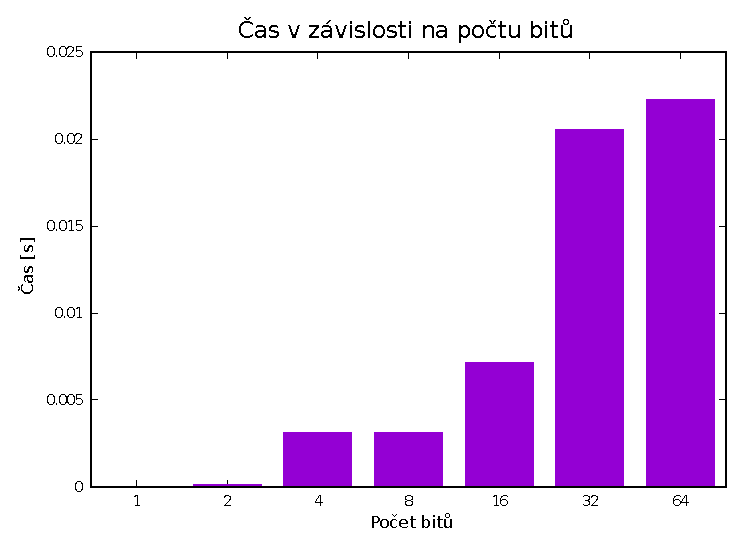
\includegraphics[width=14cm,keepaspectratio]{time.eps}

\section{Komunikační protokol}
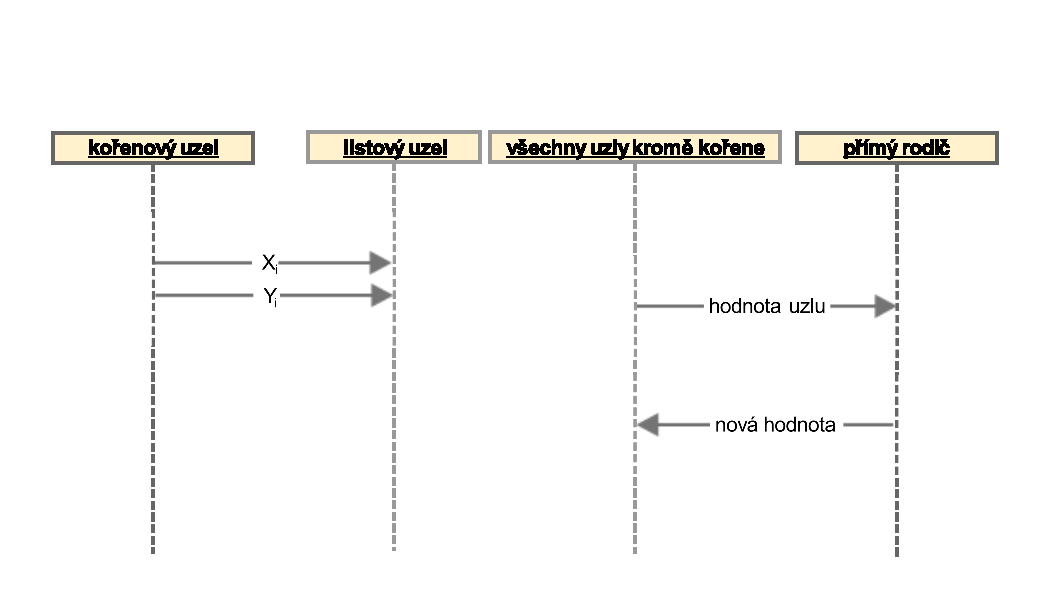
\includegraphics[width=14cm,keepaspectratio]{sequence.eps}

\section{Závěr}
\end{document}
